\section{Erstellung}
Um zu verstehen, wie Produkttesten in eine Ontologie integriert werden kann, wird anhand des Beispiels des BAYOOSOFT Access Managers eine Ontologie schrittweise aufgebaut. Die Testfälle wurde bereits im Rahmen des Praxisprojekts ermittelt und werden jetzt als Grundlage für die Ontologie verwendet. Die Ontologie wurde in Protégé entworfen und mit webVOWL visualisiert. \newline
In folgendem Beispiel werden Funktion und Testfälle des Verwaltens von Berechtigungen zunächst stark einfacht modelliert:\\

\begin{center}
    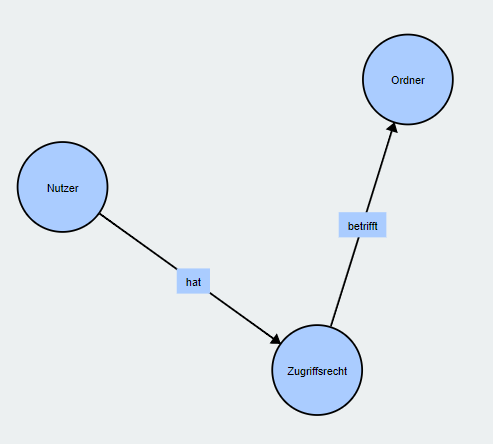
\includegraphics[width=1\textwidth]{Thesis/Images/OntologySmall.png}        
\end{center}

Die Ontologie fasst die Funktion des Berechtigungsmanagements in 3 Klassen mit 2 Beziehungen zusammen. 
%%%%%%%%%%%%%%%%%%YIKES
Verwendet man die Ontologie nun auf spezielle Ausprägungen mit den für das System bekannten Daten (Zugriffsrechte umfassen Lese- und Schreibrechte) und Testdaten wie verschiedene Nutzer oder Ordner, ergeben sich verschiedene Testfälle, die die hier dargestellte Funktionalität abdecken. So hat z.B. Nutzer A Schreibrechte auf Ordner Y, aber hat keinen Zugriff auf Ordner. \\
%%%%%%%%%%%%%%%%%%YIKES
Die gezeigte Ontologie umfasst offensichtlicherweise nicht alle Aspekte des Produkts und seiner Berechtigungsverwaltung. Im nächsten Schritt wird die Ontologie erweitert, um Sonderfälle und technische Einschränkungen zu berücksichtigen.\\

\begin{center}
    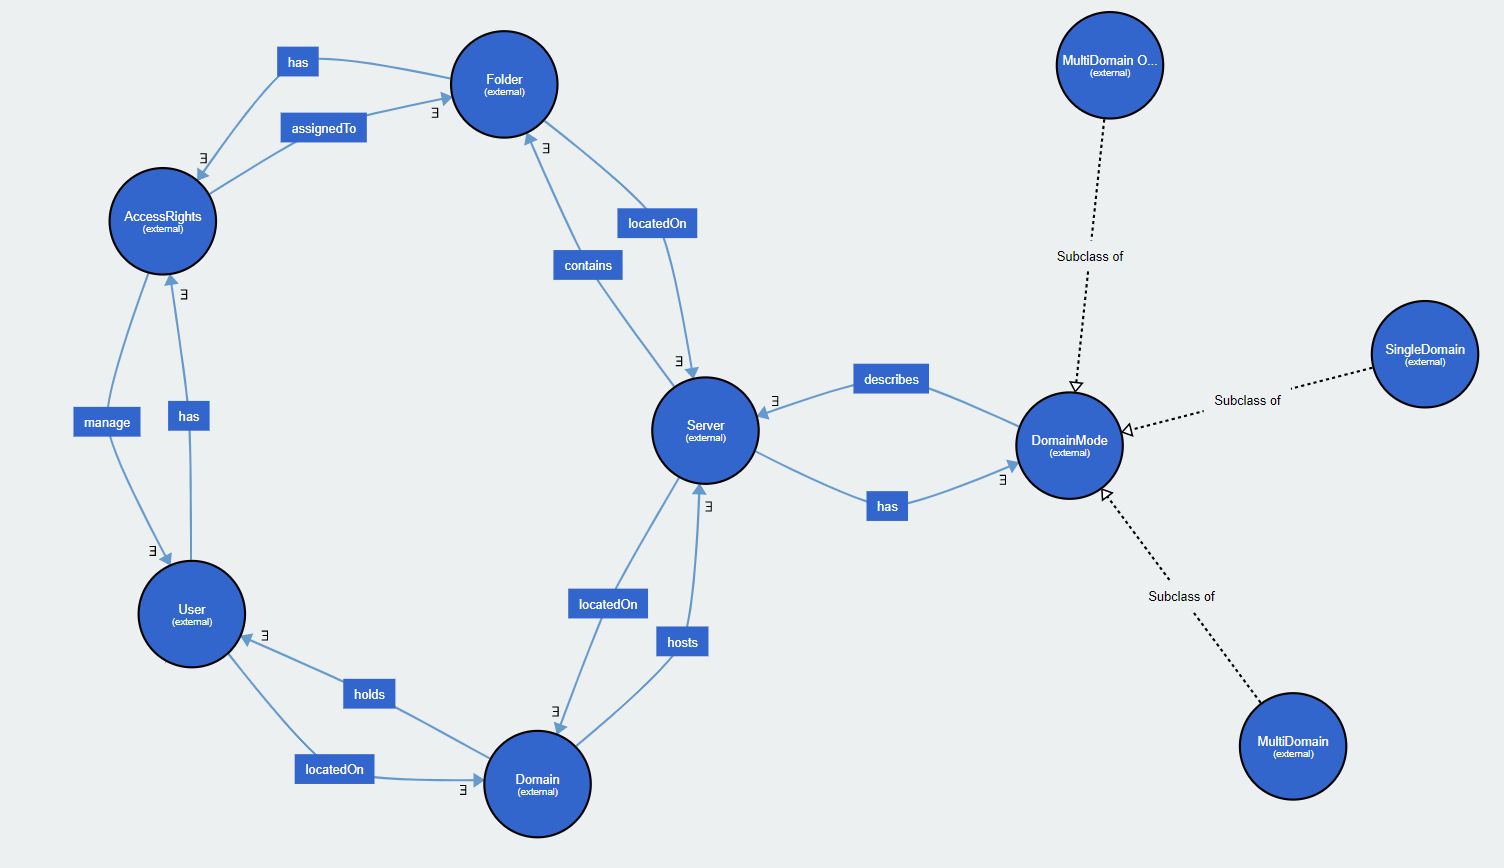
\includegraphics[width=1\textwidth]{Thesis/Images/OntologyBig.png}
\end{center}

Durch diese Erweiterungen werden in der Ontologie noch Domänen einbezogen, auf denen sich User und Ordner befinden, sowie zusätzlich Domainmodes, die jeweils entsprechend der Domäne regeln, ob ein Nutzer berechtigt werden kann oder nicht. Dadurch wird sowohl das System realitätsnaher dargestellt, als auch mehr Testfälle einbezogen.
